\subsubsection{Stick Figure Model}

Motion capture of human walking has been carried out in `Lower Limb Kinematics of Human Walking with the Medial Axis Transformation'\cite{stickfigure}, where instead of a fleshed out model such as the cardboard model, A. Bharatkumar et al used a stick figure to represent the human body. In this paper they concluded that \emph{`It is easier to track the segment angles of the thigh and leg than the actual positions of the joints'}. This makes mapping much simpler than that of the cardboard model, as there are far fewer parameters to optimise. Although they did not add explicit constraints to the model in their paper, it would be easy to add such constraints to ensure a better fit of the model to the frame. Figure~\ref{fig:stickfiguremodel} shows a full three-dimensional stick figure model, and a two-dimensional model of the thigh and calf.

\begin{figure}[H]
    \centering
    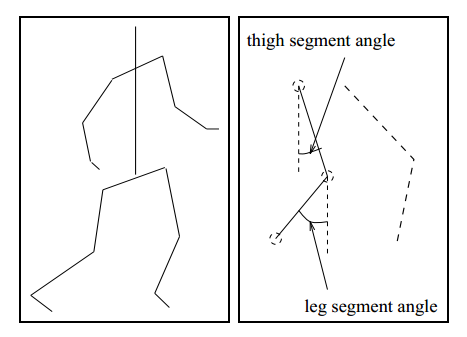
\includegraphics[height=6cm]{background/images/stickfigure}

	\caption{The stick figure model used by A. Bharatkumar et al\cite{stickfigure}}
	\label{fig:stickfiguremodel}
\end{figure}